%%%%%%%%%%%%%%%%%%%%%
%                                          %
%                 Experiment M-2           %
%         Acceleration due to gravity      %
%                                          %
%%%%%%%%%%%%%%%%%%%%%

\labChapter{M}{Acceleration due to Gravity, \textit{g}, with Glider on Tilted Air Track}

\label{lab:M2}

%\section{Introduction}
\section{Background}



By measuring the acceleration of a mass moving under the influence of the gravitational attraction of the earth, namely its weight, we can determine the acceleration due to gravity, usually denoted by $g$.  The mass will be allowed to accelerate down a presumed frictionless, inclined plane.  Measurement of the acceleration along the plane is directly related to the acceleration due to gravity by a simple trigonometric relationship.  The use of the plane permits the convenient measurement of a small, measurable fraction of the acceleration due to gravity.  This of course is in lieu of the much more difficult measurement of a vertically falling mass.














Near the surface of the earth, the attractive force of the earth on a mass can be considered a constant over a reasonable range of elevation. This force is commonly called the weight of the object and from Newton's Second Law the weight is the mass, $m$, times the acceleration due to gravity. Using Fig.~\ref{M02Fig01}. and the derivation following, we can see that the value of $g$ can be easily determined by a few simple measurements.

\begin{figure}
  \begin{center}  
    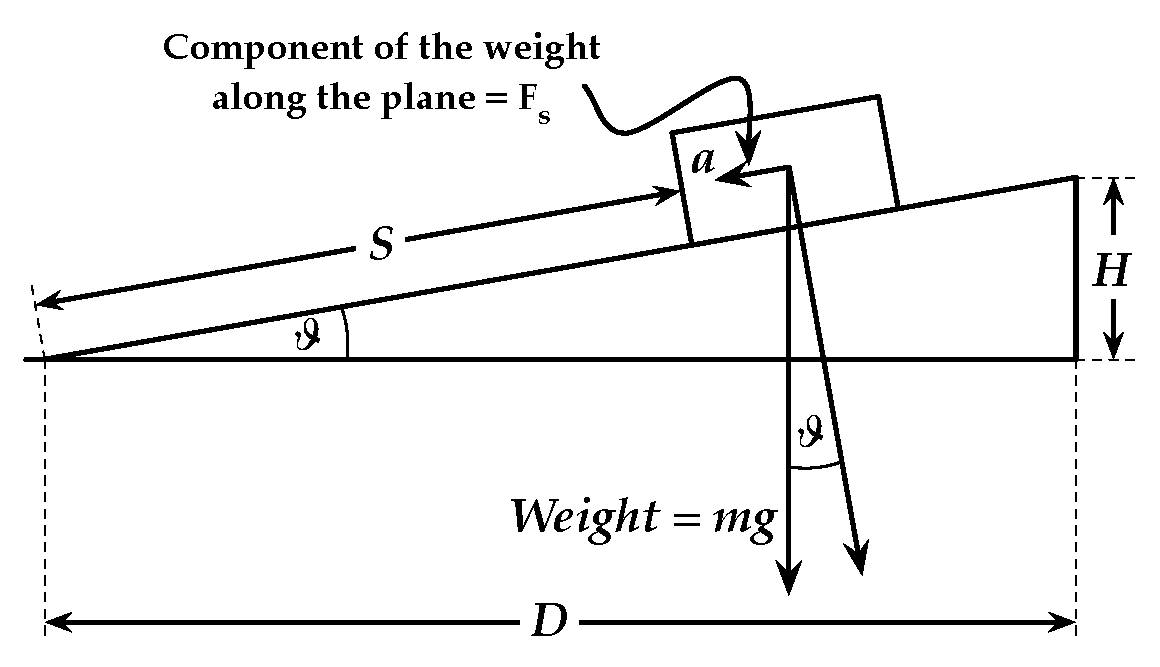
\includegraphics[width=5.5in]{Experiment02Figures/Figure01.pdf}
  \end{center}
  \caption{Force Diagram and variables used in Experiment M-\ref{lab:M2}.}
  \label{M02Fig01}  % the \label command comes AFTER the caption
\end{figure}

The displacement along the track is $S$ and the component of acceleration $a_s$ along the track is
\[
a_s = \frac{F_s}{m} = \frac{m g \sin(\theta)}{m} =  g \sin(\theta).
\]
If the mass is released from rest near the top of the inclined air track and allowed to accelerate down the air track with a magnitude $a_s$, then by measuring the transit time down the track over a measurable distance, $S$, we can determine the value of $g$.

Since the acceleration $a_s$ is constant, the displacement $S$ as a function of time $t$ is:
\[
  S = \frac{1}{2} a t^2 = \frac{1}{2} g t^{2} \sin(\theta).
\]
Solving for $g$, we obtain
\begin{equation}
  g = \frac{2 S}{t^2 \sin(\theta)}.
\end{equation}

If we assume that the incline angle $\theta$ is small, we can approximate the $\sin(\theta)$ by the $\tan(\theta) = \nicefrac{H}{D}$.
Making this substitution for the $\sin(\theta)$, we have the value of $g$ in terms of easily measurable quantities, namely
\begin{equation}
  \label{eq:M02gvalue}
  g = \frac{2 S D}{H t^2}
\end{equation}
where $H$ is the vertical rise in the horizontal distance $D$.  $D$ is the distance between the legs of the air track, and $t$ is the transit time of the mass, starting from zero velocity and accelerating down the plane a distance $S$ along the plane.
We will compare our results to the measured value of $g$ at sea level.  The value at sea level at New York is $g = 9.803\,\meter\per\second\squared$.

In the experiment, the presumed frictionless inclined plane will be an air track.  The mass will be a glider, which floats on the air track.  Placing a spacer of height $H$ under the leg at one end of the track, which is a distance $D$ from the leg(s) at the opposite end, will incline the track.  Refer to Fig.~\ref{M02Fig02} below in the experimental procedure section.

%\subsection{Acceleration by a hanging mass}
% --- removing, doesn't necessarily incorporate torque, doesn't add much to the lab at this point - 2024/08

%In this case you will use the \textbf{Capstone} program and the PASCO rotary sensor to measure $g$.
%Set the track level, with no spacer.
%The glider has mass $M_G$.
%A string connects the glider with a weight of mass $M_w = 10\,\gram$.
%The string passes over the large pulley of a PASCO rotary sensor.
%You have to account for the  mass of the rotating pulley to get a more accurate result.
%Your measured value for $g$ is found from
%\begin{equation}
%\label{eq:M2hanging}
%  M_w g = \left(M_G + M_{pulley} + M_w\right) a.
%\end{equation}
%Here $\left(M_G + M_{pulley} + M_w\right)$ is the total mass that is moving and $M_w g$ is the total force.
















\section{Experimental Procedure}

\begin{figure}[ht]
  \begin{center}
    %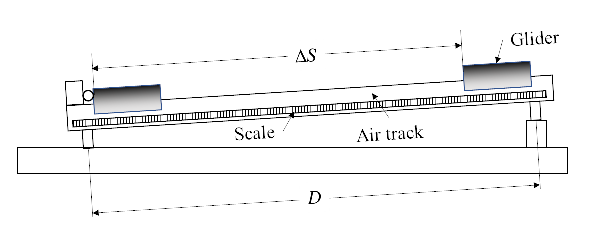
\includegraphics[width=5.6in]{Experiment02Figures/Figure02.eps}
    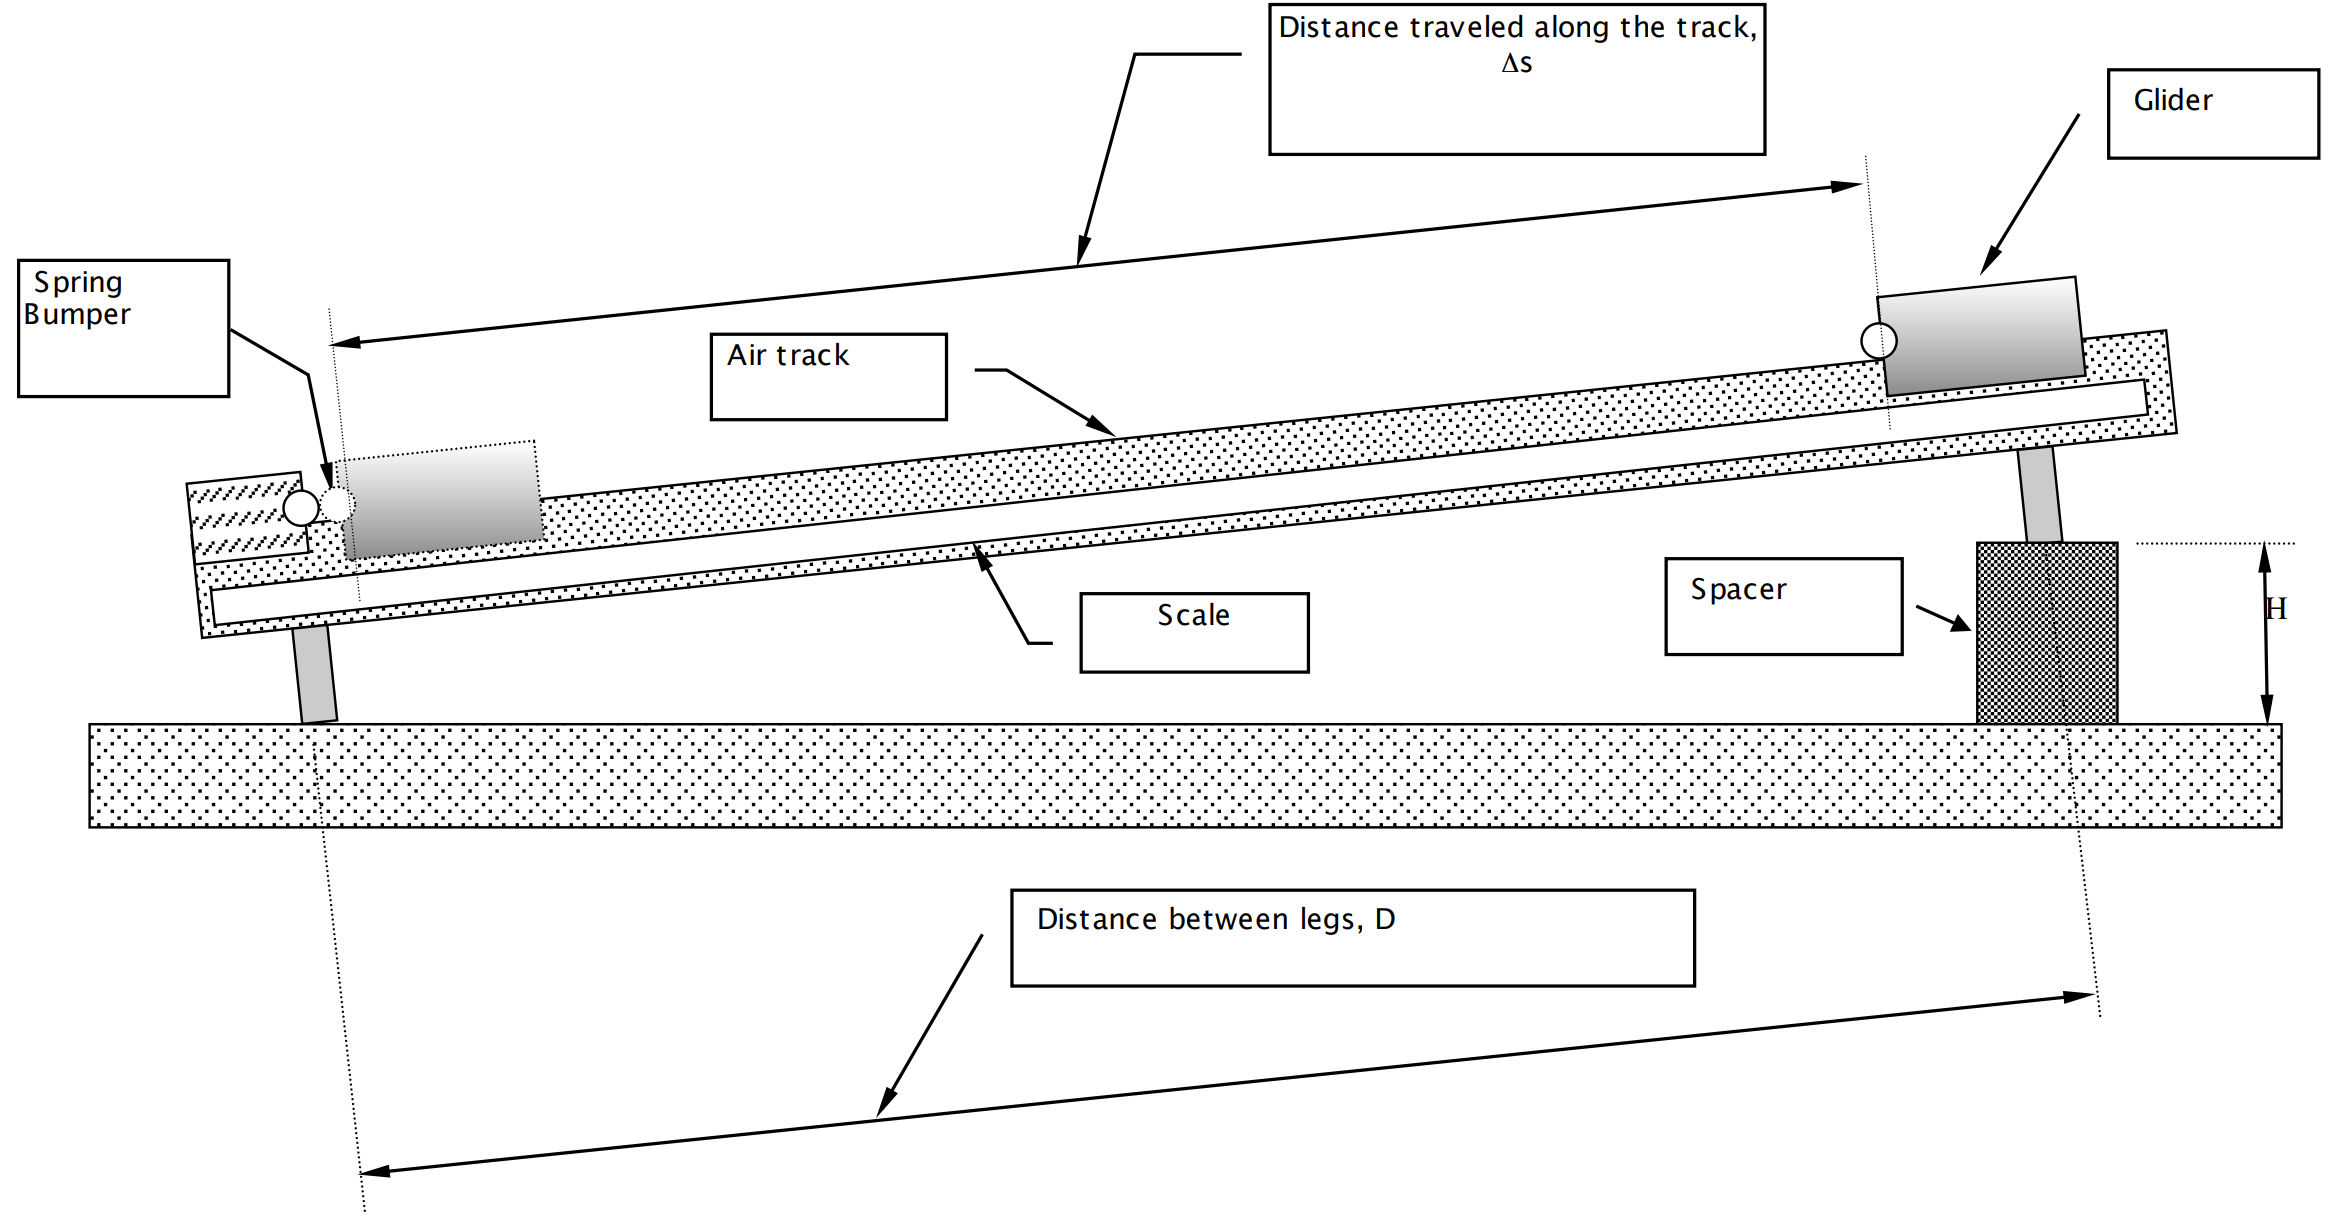
\includegraphics[width=5.8in]{Fall/Experiment02Figures/M02_fig2.png}
  \end{center}
  \caption{Experimental Setup for M-\ref{lab:M2}.}
  \label{M02Fig02}
\end{figure}

In this experiment you will measure the motion of a glider down a tilted track using PASCO photogates (stated precision of 0.0001 seconds) connected to PASCO's data logging and visualization software, \textbf{Capstone}, which will be set up as a timer for this experiment. 
\begin{enumerate}
\item %Turn on the air and allow it to run a couple of minutes before proceeding. It is very important that the track is clean and free of dirt. This will prevent any damage to the very expensive air track and will keep friction to an absolute minimum. 
\textbf{\textit{Do not put a glider on the track without air flowing.}}
\item Create a table of the common data including the masses of the gliders, the distance $D$ between the legs of the air track and the heights of the two spacers.
\item Measure and record the mass of both the large and small glider.
\item Without the spacer present and the air track resting directly on the tabletop (with the black circle feet), place one of the gliders on the track and note any preferential drift of the glider.  Adjust the height of the single leg (screw in or out) until the air track is level, as indicated by no preferential drift.  Check both orientations of the glider on the track to check if the car is asymmetric and has a significant preferential drift on an otherwise level track.  If this occurs, use another glider.
\item Measure and record the distance $D$.  This is the center-to-center distance between the legs.
\item Measure and record the heights, $H$, of each of the two spacers with the provided Vernier caliper for greater precision.
\item Four cases will be performed with a tilted air track, two gliders with two spacers (e.g. BIG spacer/small glider, BIG spacer/BIG glider, small spacer/small glider, small spacer/BIG glider).
%The final case will use a hanging mass to accelerate the glider.  
\item Determine a convenient point on the glider to use with the scale attached on the side of track.  It doesn't matter what point you choose, only that you use the same point for all determinations of $\Delta s$ for that glider.  A convenient point is the lower front or rear corner of the glider since it will be very close or overlapping with the length scale on the track itself.
%\item For each of the first four cases, perform the following steps and record the data appropriately in your spreadsheet:
\item For each of the four cases, perform the following steps and record the data appropriately in your spreadsheet:
  \begin{enumerate}
  \item For each of the four cases with a tilted track create enough \textbf{rows} for the number of trials you are doing, and \textbf{columns} for each of the variables you will be measuring or deriving:
    \begin{itemize}
      \item starting point at the top $s_1$
      \item stopping point at the bottom $s_0$
      \item distance between the photogates that the glider travels $S$
      \item start time at the top $t_1$
      \item time at the bottom $t_0$
      \item time between the photogates $\Delta t$
      \item calculated value of $g$ using Eqn.~\ref{eq:M02gvalue} for each of the five trials
      \item average value of $g$ from the five trials of each case
      \item standard deviation of $g$ from the five trials of each case
      \item difference between the average value of $g$ and the accepted value of $9.803\,\meter\per\second\squared$ for Fairfield, CT for each case
      \item similarly, the average, standard deviation, and difference for $g$ from all 20 trials across all 4 cases
      \end{itemize}
  \item Raise the single leg side of the track by placing a spacer under the knob.
  %\item Place the glider at the bottom of the track resting against the bumper. Record $s_{0}$. (Note: With the car at this position, the red light on the bottom photogate should be lit. Moving the glider to the right the slightest distance should put the light out. If this is not the case, adjust the position of the photogate.)
  \item Place the glider near the bottom of the track. Move it slowly as you approach the bottom photogate. Stop the glider at the exact location when the photogate's red light comes on. Record position on the scale, $s_0$.
  \item Next, place the glider near the top of the track. Move it slowly as you approach the top photogate. Stop the glider at the exact location when the photogate's red light comes on. Record position on the scale, $s_1$.
  %\item Before you take the recorded data in the next step, take some practice runs. Your subsequent data will be much improved by your training! Set the photogate timer to pulse mode. Position the glider so it is blocking the top photogate and the red light is on. Place one finger on the track in front of the glider and gently push the glider to the right until the red light on the photogate just goes out. Press the reset button on the timer. Release the glider by quickly pulling your finger away from the track. After the glider bounces off the lower bumper, the time of travel from top to bottom will be displayed on the timer.
  \item Before you take the recorded data in the next step, take some practice runs. Your subsequent data will be much improved by your training! Press record in \textbf{Capstone} to start the timer. \textit{NOTE: }\textbf{Capstone} will display the time whenever a photogate beam is broken; the time at the higher (start) photogate $t_1$ as well as the time at the lower (end) photogate $t_0$. To determine the total transit time $\Delta t$, take the difference of the start and end times.
  \item Position the glider so it is blocking the top photogate and the red light is on. Place one finger on the track in front of the glider and gently move the glider up the track (to the right) until the red light on the photogate just goes out.
  \item Release the glider by quickly pulling your finger away from the track and glider (MINIMIZE ANY FINGER CONTACT WITH THE GLIDER to minimize any additional push or pull on the glider to \textbf{ensure its initial velocity is zero}). 
    \item For each of the \textbf{5 trials per case}, release the glider from rest at the $s_1$ position. Measure and record the start time $t_1$ and end time $t_1$ to determine transit time $\Delta t$ from release at the top to bottom of the airtrack. Calculate the value of $g$ for this trial.
















    
  \end{enumerate}





  \item For each the four cases:
\begin{itemize}

  \item Calculate the average of the measured $g$
  \item Calculate the standard deviation of the measured $g$
  \item Calculate the differences between your average $g$ and the accepted value of $g$
  %\item Create a new table for the acceleration of the glider with the hanging mass.  including:
  %  \begin{itemize}
  %    \item the glider $M_G$, the pulley $M_{pulley}$, and the hanging weight $M_w$ masses,
  %    \item the acceleration $a_G$ of the glider,
  %    \item the experimental value of $g$ using Eqn.~\ref{eq:M2hanging}.
  %  \end{itemize}
\end{itemize} 

  \item Also, using data from all trials from all the cases:
  \begin{itemize}
    \item Calculate the average of the measured $g$.
    \item Calculate the standard deviation of the measured $g$.
    \item Calculate the differences between your average $g$ and the accepted value of $g$
  \end{itemize}

\end{enumerate}

%The next experiment is performed by accelerating the glider along a level track with a hanging weight.  You will use the Capstone program and the PASCO rotary sensor. 
%\begin{itemize}
%\item Remove the spacers and return the track to level. 
%\item Turn on the air and allow it to run a couple of minutes before proceeding. It is very important that the track is clean and free of dirt. This will prevent any damage to the very expensive air track and will keep friction to an absolute minimum. Do not put a glider on the track without air flowing.
%\item Attach the string provided to red glider with mass $M_G$.
%Pass the string over the large pulley of the rotary sensor.
%Hang a $M_w = 10$ gram weight on the string.
%\item Pull the glider along the track until the hanging weight is near the pulley and hanging freely.
%\item Start recording using the \textbf{Capstone} program. See page~\ref{sec:SettingUpHardware}.
%\item Release the glider. The mass will fall, rotate the pulley and pull the glider.
%\item Stop recording once the glider hits the end of the track.
%\item Record the slope of the line which is the acceleration $a_G$ of the glider. Calculate $g$ using Eqn.~\ref{eq:M2hanging} with $M_{pulley} = 6\,\gram$.
%\end{itemize}












%\section{Data Analysis}













\section{Post-Lab Submission --- Interpretation of Results}

\begin{itemize}

\item Make sure to submit your finalized data table (Excel sheet)

\item If you release the glider higher above the photogate rather than right at the gate, what would you expect to happen to your derived values of $g$? 
\item What are sources of uncertainty (initial v, friction, etc.)?
\item What was the precision of the instrumentation (e.g. caliper, time, distance, etc.)?
\item Compare your results ($g$ from each of the four cases and one from all 20 trials) to the accepted value. How do the standard deviations compare to the difference between your values of $g$ and the accepted value of $g$? I.e. while treating the standard deviations of your measurements as your measurement uncertainties, do your values of $g$ for each case, as well as the overall average $g$, plus or minus the standard deviations overlap (and agree) with the accepted value of $g$? What might cause your results to disagree the most?
\item Suppose there is a frictional force slowing the glider as it moves along the track. How would this affect the determined value of $g$? Would your result support or not support the hypothesis of that there is significant friction along the track?
\item Assume the track is not level at the beginning of the experiment. Further, assume that what you thought to be a level track was in fact slightly tipped in the same direction as your deliberate tipping via the spacers during the experiment. How would this affect the determined value of $g$? Would your result support or not support the hypothesis of the track not being level?



%\item Calculate the average value of $g$ from all your measurements and determine the difference between your result and the commonly accepted value of $9.803\,\meter\per\second\squared$.
%\item Suppose there is a frictional force slowing the glider as it moves along the track. Explain the effect on the measurement of the value of $g$ and state whether your result would support the hypothesis of friction along the track.
\end{itemize}

